\documentclass[11pt,a4paper]{ctexart}

\usepackage[a4paper,margin=2.15cm,headheight=15pt]{geometry}
\usepackage{amsmath,amssymb}
\usepackage{graphicx}
\usepackage{booktabs}
\usepackage{tabularx}
\usepackage{array}
\usepackage{xcolor}
\usepackage{float}
\usepackage{caption}
\usepackage{enumitem}
\usepackage{fancyhdr}
\usepackage{hyperref}
\usepackage{pdflscape}

\definecolor{pandaxblue}{HTML}{1F5A7A}
\definecolor{pandaxgreen}{HTML}{2A8F55}
\definecolor{softgray}{HTML}{F2F5F7}
\definecolor{warnorange}{HTML}{C56A18}

\hypersetup{
  colorlinks=true,
  linkcolor=pandaxblue,
  urlcolor=pandaxblue,
  pdftitle={PandaX-4T 老师反馈后的模型完善与结果汇报},
  pdfauthor={PandaX 能量重建项目}
}

\pagestyle{fancy}
\fancyhf{}
\lhead{\textcolor{pandaxblue}{PandaX-4T 能量重建}}
\rhead{\textcolor{gray}{candidate\_v10}}
\cfoot{\thepage}

\setlength{\parindent}{2em}
\setlength{\parskip}{0.35em}
\setlist[itemize]{leftmargin=2em,itemsep=0.25em}
\setlist[enumerate]{leftmargin=2.2em,itemsep=0.3em}
\captionsetup{font=small,labelfont=bf}
\newcommand{\var}[1]{\texttt{\detokenize{#1}}}
\newcommand{\pass}{\textcolor{pandaxgreen}{\textbf{PASS}}}

\begin{document}

\begin{titlepage}
  \centering
  \vspace*{2.2cm}
  {\Huge\bfseries\color{pandaxblue}
  PandaX-4T 能量重建模型完善与结果汇报\par}
  \vspace{0.8cm}
  {\Large 根据老师反馈完成的一维、二维与关键变量分析\par}
  \vspace{1.4cm}
  \rule{0.78\textwidth}{1.1pt}
  \vspace{1.2cm}

  \begin{tabular}{rl}
    数据：& Run 10972，4499 个有效事件，985 个采集文件\\
    当前候选：& sparse candidate\_v10\\
    模型：& spline basis + Ridge，平滑修正上限 0.10\\
    验证：& 连续文件块、嵌套选参、12 种峰拟合协议\\
    日期：& 2026 年 7 月 31 日
  \end{tabular}

  \vfill
  \begin{minipage}{0.86\textwidth}
    \colorbox{softgray}{
      \parbox{0.92\textwidth}{
      \textbf{本次工作的核心结论：}
      在保持完整采集文件隔离的前提下，模型由 30 个变量减少到 20 个；
      五个未见文件块上均优于当前线性公式和已有三次多项式
      \var{Energy_cor}。外层文件块的
      $\sigma/\mu$ 中位数由已有修正的 $4.301\%$ 降至 $2.573\%$。
      该结果仍属于 Run 10972 内部验证，不能替代独立新 run 盲测。
      }
    }
  \end{minipage}
\end{titlepage}

\tableofcontents
\clearpage

\section{老师反馈与本次任务}

老师在聊天中提出了四项明确要求：

\begin{enumerate}
  \item 变量越少越容易控制，应尝试减少变量数量；
  \item 比较我们的 corrected energy 与已有 corrected energy；
  \item 给出一维直方图和二维 $x$--$y$ 对比；
  \item 检查变量修正前后的变化趋势，并找出最关键的几个变量。
\end{enumerate}

本次工作没有仅在完整数据上删除变量，而是把“变量数量”和“变量身份”放入嵌套验证。
因此，外层测试文件块既不参与变量排序，也不参与变量数量选择。

\begin{table}[H]
\centering
\caption{老师要求与本次交付内容的对应关系}
\begin{tabularx}{\textwidth}{>{\bfseries}p{0.24\textwidth}X>{\centering\arraybackslash}p{0.12\textwidth}}
\toprule
老师要求 & 本次实现 & 状态\\
\midrule
减少变量 & 在 $k=3,5,8,12,20,30$ 中进行训练侧嵌套选择 & \pass\\
一维能谱对比 & 当前线性、已有三次多项式、v10 三路线同图比较 & \pass\\
二维 $x$--$y$ 对比 & 逐事件位置散点，以能量偏差着色 & \pass\\
变量变化趋势 & 对前四个关键变量绘制等计数分箱趋势 & \pass\\
关键变量 & 给出重要性、外层入选次数和物理类别 & \pass\\
其他 run & 当前尚未获得并运行独立新 run & 待完成\\
\bottomrule
\end{tabularx}
\end{table}

\section{比较对象与统一评价口径}

\subsection{当前线性组合}

当前基础能量方向为
\begin{equation}
E_0=
\frac{qS1ub\_C}{0.125}
+\frac{qS2Bdesub\_C}{10.58}.
\end{equation}
峰宽评价对整体常数缩放不敏感；为比较峰中心，所有外层折的标定常数均只由该折训练侧产生。

\subsection{已有三次多项式 corrected energy}

老师要求比较的已有修正写为
\begin{align}
E &=0.0137\left(
\frac{qS1ub\_C}{0.125}
+\frac{qS2Bdesub\_C}{10.58}
\right),\\
E_{\mathrm{cor}}^{\mathrm{legacy}}
&=-1.73706\times10^{-9}E^3
+7.98193\times10^{-6}E^2
+1.07904E-9.22086.
\end{align}

为了避免测试块峰中心泄漏，图表中的 legacy 路线也只使用对应训练文件块给出的固定尺度，
测试侧不重新对齐峰中心。

\subsection{统一峰宽指标}

主指标为 12 种预先固定峰拟合协议下的中位数
\begin{equation}
R_{\mathrm{fit}}
=\operatorname{median}_{p\in\mathcal P}
\left(\frac{\sigma_p}{\mu_p}\right),
\qquad |\mathcal P|=12.
\end{equation}
同时报告稳健宽度
\begin{align}
R_{68}&=\frac{Q_{84.135}-Q_{15.865}}{2Q_{50}},\\
R_{90}&=\frac{Q_{95}-Q_{5}}{2Q_{50}}.
\end{align}
这样可以避免只依赖一个有利的拟合窗口。

\section{稀疏 candidate\_v10}

\subsection{模型形式}

v10 保留 v9 的平滑低容量路线。对每个环境变量构造有限的三次样条基函数，
再使用 Ridge 回归预测基础能量的对数偏差：
\begin{equation}
\widehat{\delta}_{\mathrm{raw}}(\mathbf x)
=\boldsymbol\beta^{\mathsf T}\boldsymbol\phi(\mathbf x).
\end{equation}

为了避免硬截断产生边界堆积，修正采用
\begin{equation}
\widehat{\delta}
=c\tanh\left(
\frac{\widehat{\delta}_{\mathrm{raw}}}{c}
\right),
\qquad c=0.10,
\end{equation}
最终能量为
\begin{equation}
E_{\mathrm{v10}}
=K E_0\exp(-\widehat{\delta}),
\end{equation}
其中 $K$ 只由当前训练侧确定。

\subsection{数据隔离}

Run 10972 按 \var{fileNumber} 划分为五个连续完整文件块：
\[
[0,200),\ [200,400),\ [400,600),\ [600,800),\ [800,1000).
\]
\var{fileNumber} 只用于分组、审计和稳定性检查，不进入预测器。
每轮留下一个完整文件块作为外层测试，其余文件块内部再完成变量排序与 $k$ 的选择。

\subsection{变量数量不是人工指定}

\begin{figure}[H]
\centering
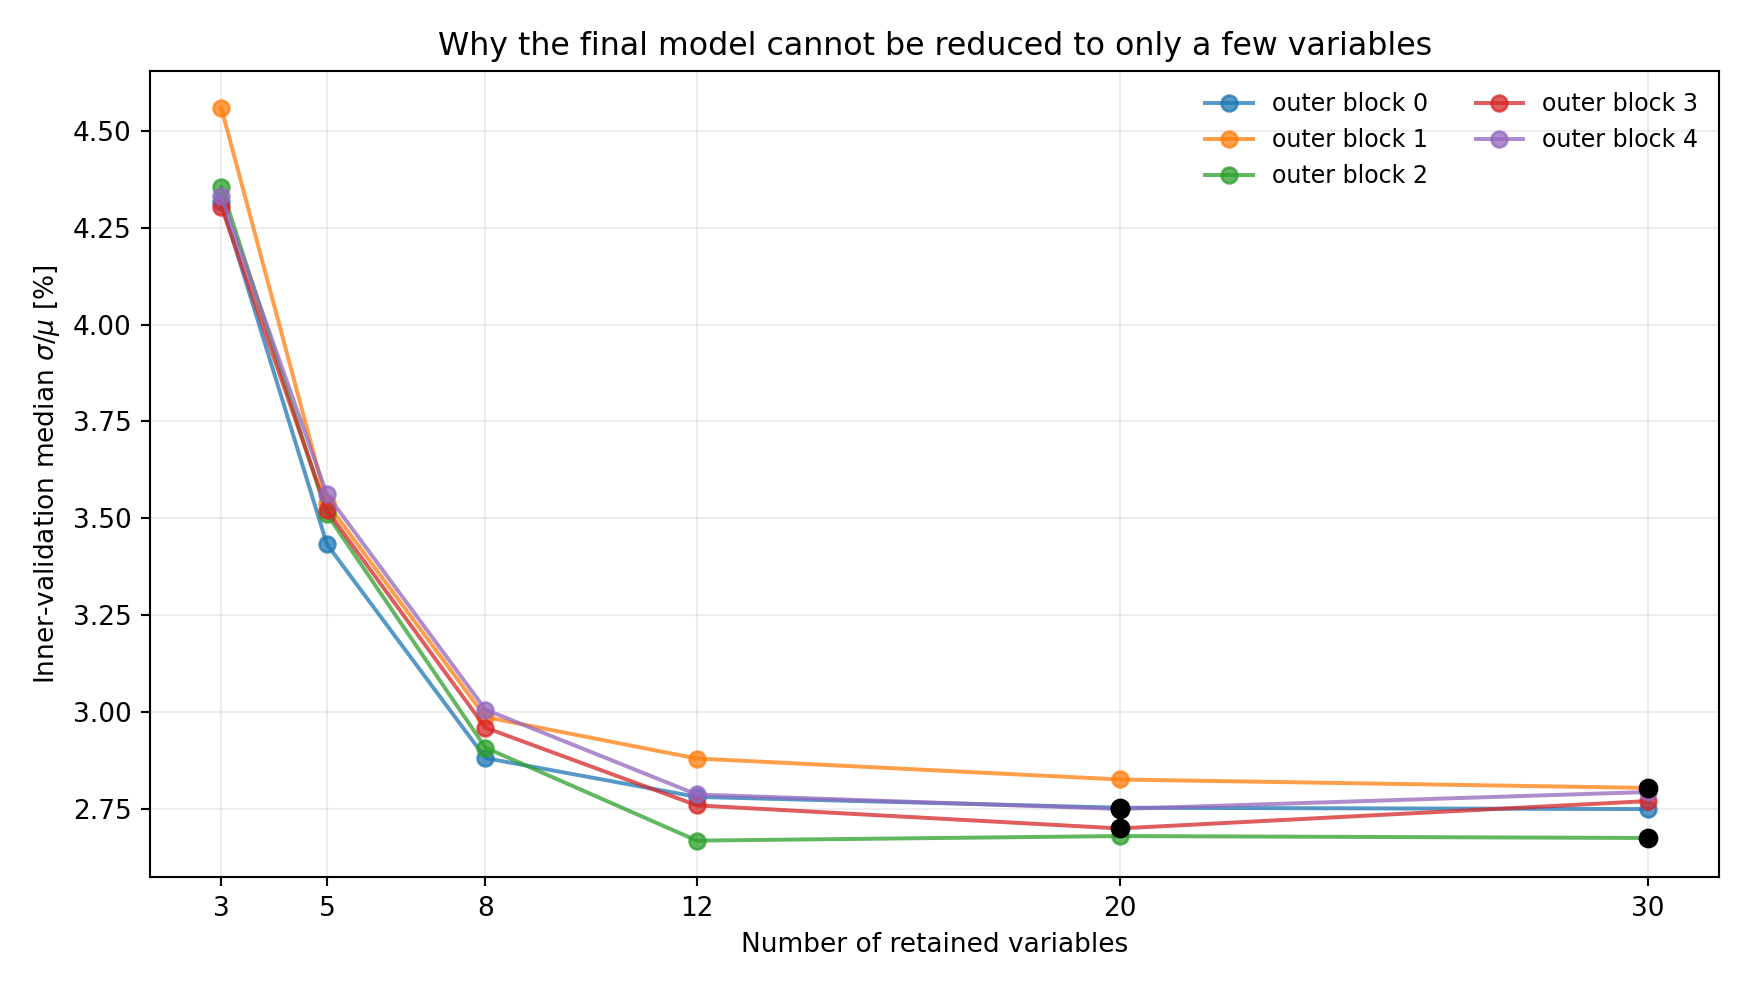
\includegraphics[width=0.96\textwidth]{figures/variable_count_selection.png}
\caption{不同变量数量在内层未见文件块上的表现。每条彩色曲线对应一个外层训练池；
黑点表示该外层流程最终选择的变量数量。}
\end{figure}

图中可以看到：
\begin{itemize}
  \item 只使用 3 个变量时，内层 $\sigma/\mu$ 约为 $4.3\%$--$4.6\%$；
  \item 5 个变量仍约为 $3.4\%$--$3.6\%$；
  \item 8 个变量后进入约 $2.9\%$--$3.0\%$；
  \item 12 个变量后改善趋缓；
  \item 20 与 30 个变量处于性能平台。
\end{itemize}

五个外层训练池分别选择
\[
20,\ 30,\ 30,\ 20,\ 20
\]
个变量。完整训练阶段最终选择 20 个变量，相比 v9 的 30 个变量减少
\[
\frac{30-20}{30}=33.3\%.
\]
因此，本次结果支持“减少到 20 个”，但不支持为了方便控制而强行压缩到 3--8 个。

\section{关键变量}

\begin{landscape}
\begin{figure}[H]
\centering
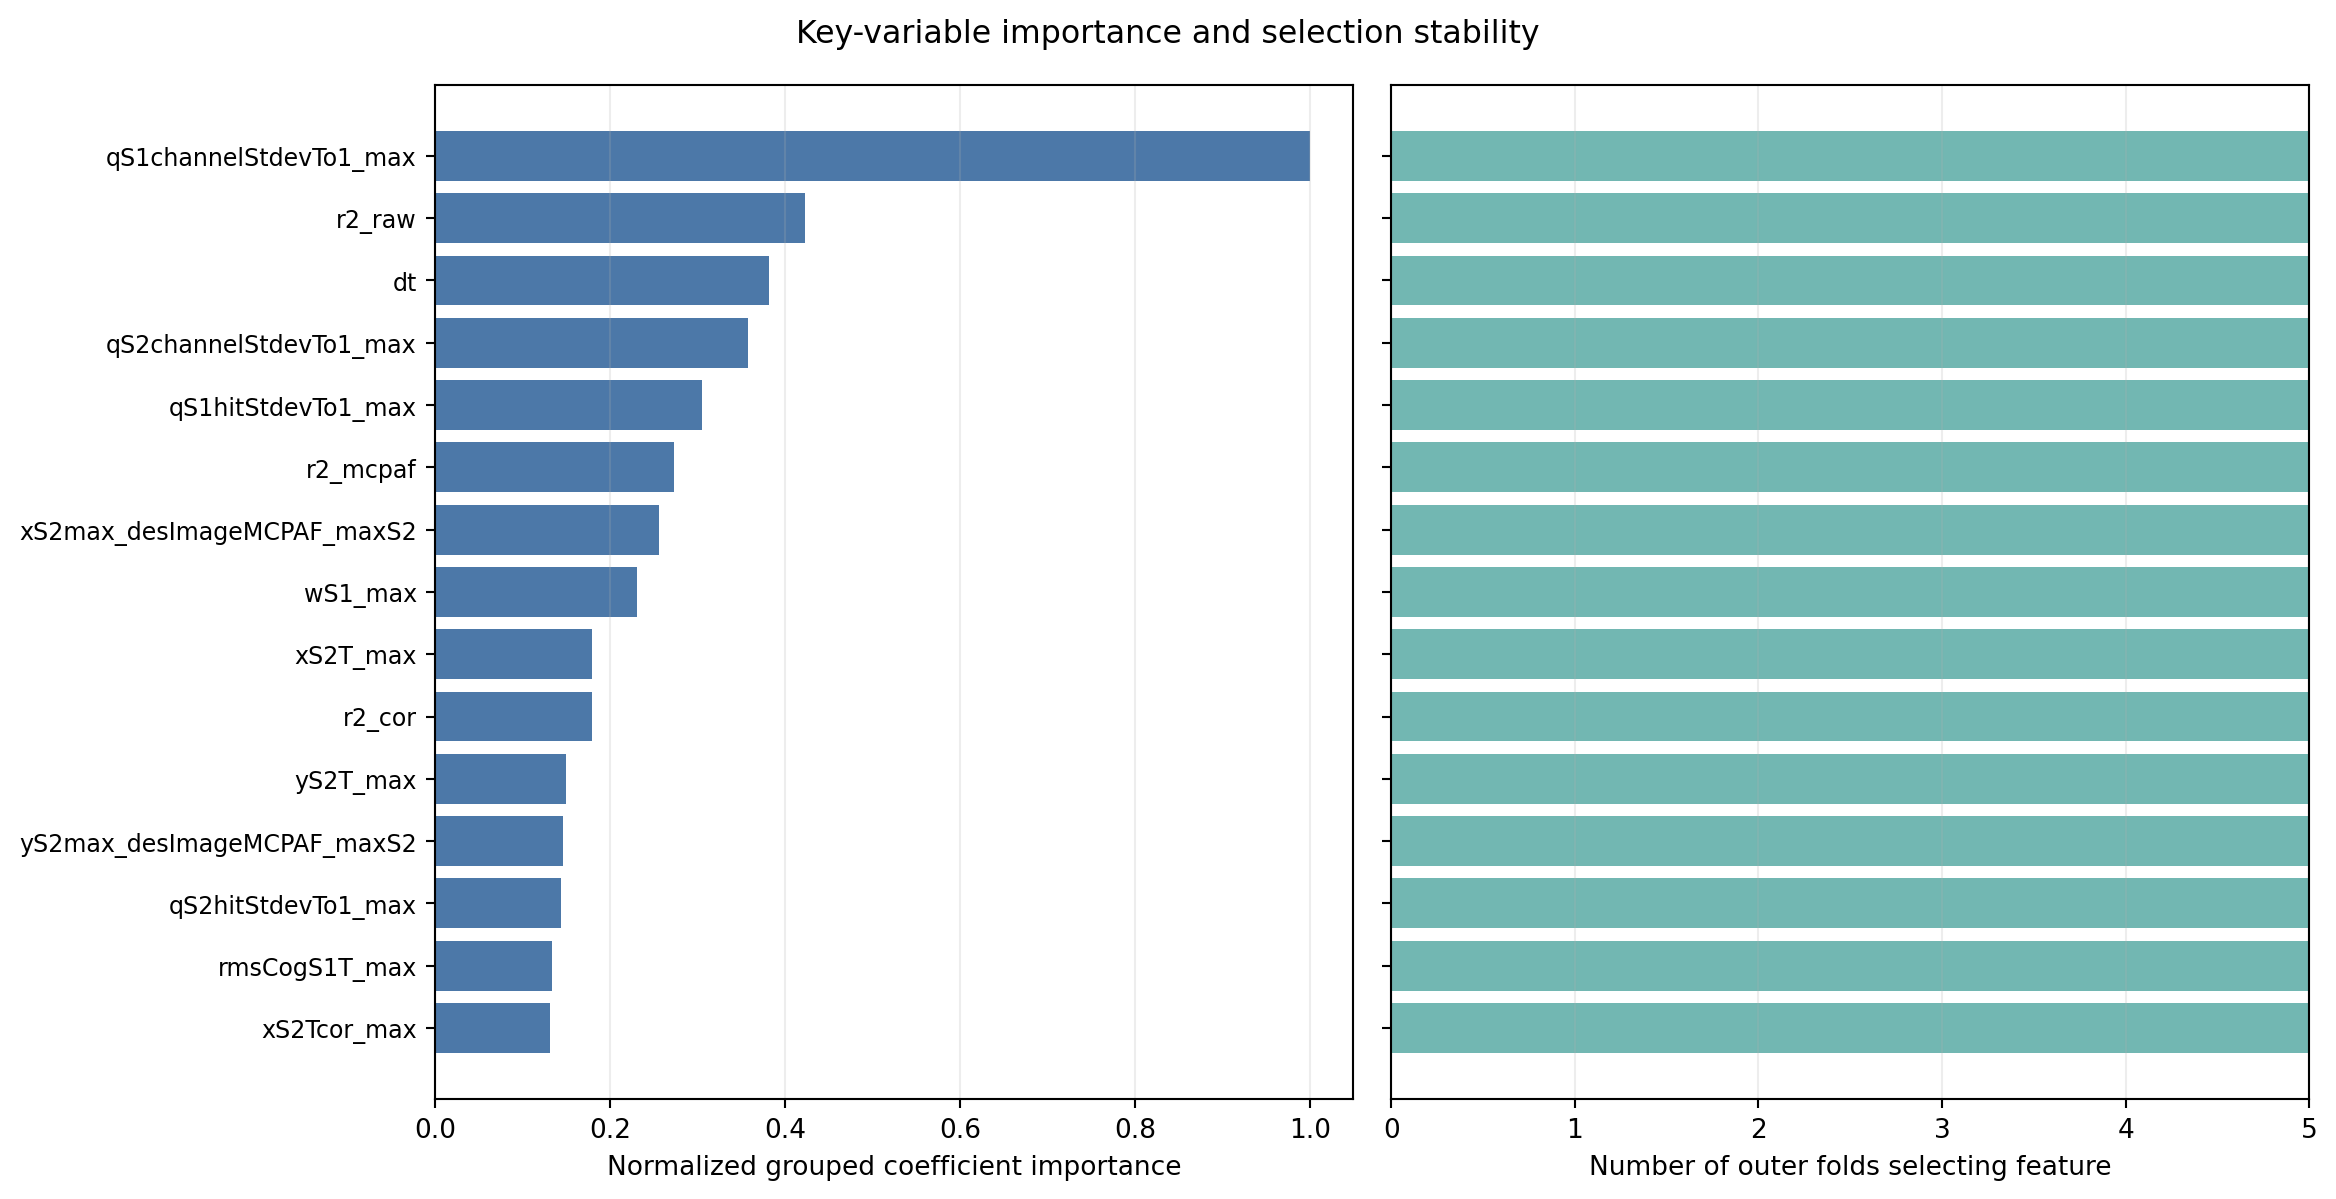
\includegraphics[width=0.94\linewidth]{figures/feature_importance.png}
\caption{左：全量冻结模型中的分组样条系数重要性；右：该变量在五个外层训练流程中的入选次数。
重要性用于排序，不解释为唯一因果贡献。}
\end{figure}
\end{landscape}

排名最高且五个外层折全部入选的前五个变量为：

\begin{table}[H]
\centering
\caption{最关键的五个变量}
\begin{tabularx}{\textwidth}{c>{\ttfamily}p{0.34\textwidth}Xc}
\toprule
排名 & \normalfont 变量 & 可支持的物理解释 & 外层入选\\
\midrule
1 & qS1channelStdevTo1\_max & S1 通道响应离散程度的代理量，可能反映光收集与通道图样非均匀性 & 5/5\\
2 & r2\_raw & 原始横向重建半径平方，反映中心与边缘的空间响应差异 & 5/5\\
3 & dt & 漂移时间或纵向位置代理，反映电子漂移与深度相关响应 & 5/5\\
4 & qS2channelStdevTo1\_max & S2 通道响应离散程度的代理量，反映电荷图样与局部响应差异 & 5/5\\
5 & qS1hitStdevTo1\_max & S1 hit 级离散程度的代理量，补充通道图样信息 & 5/5\\
\bottomrule
\end{tabularx}
\end{table}

这里必须保持谨慎：上述解释是变量类别层面的响应代理，不等价于证明某个变量是能量偏差的微观因果来源。

\begin{figure}[H]
\centering
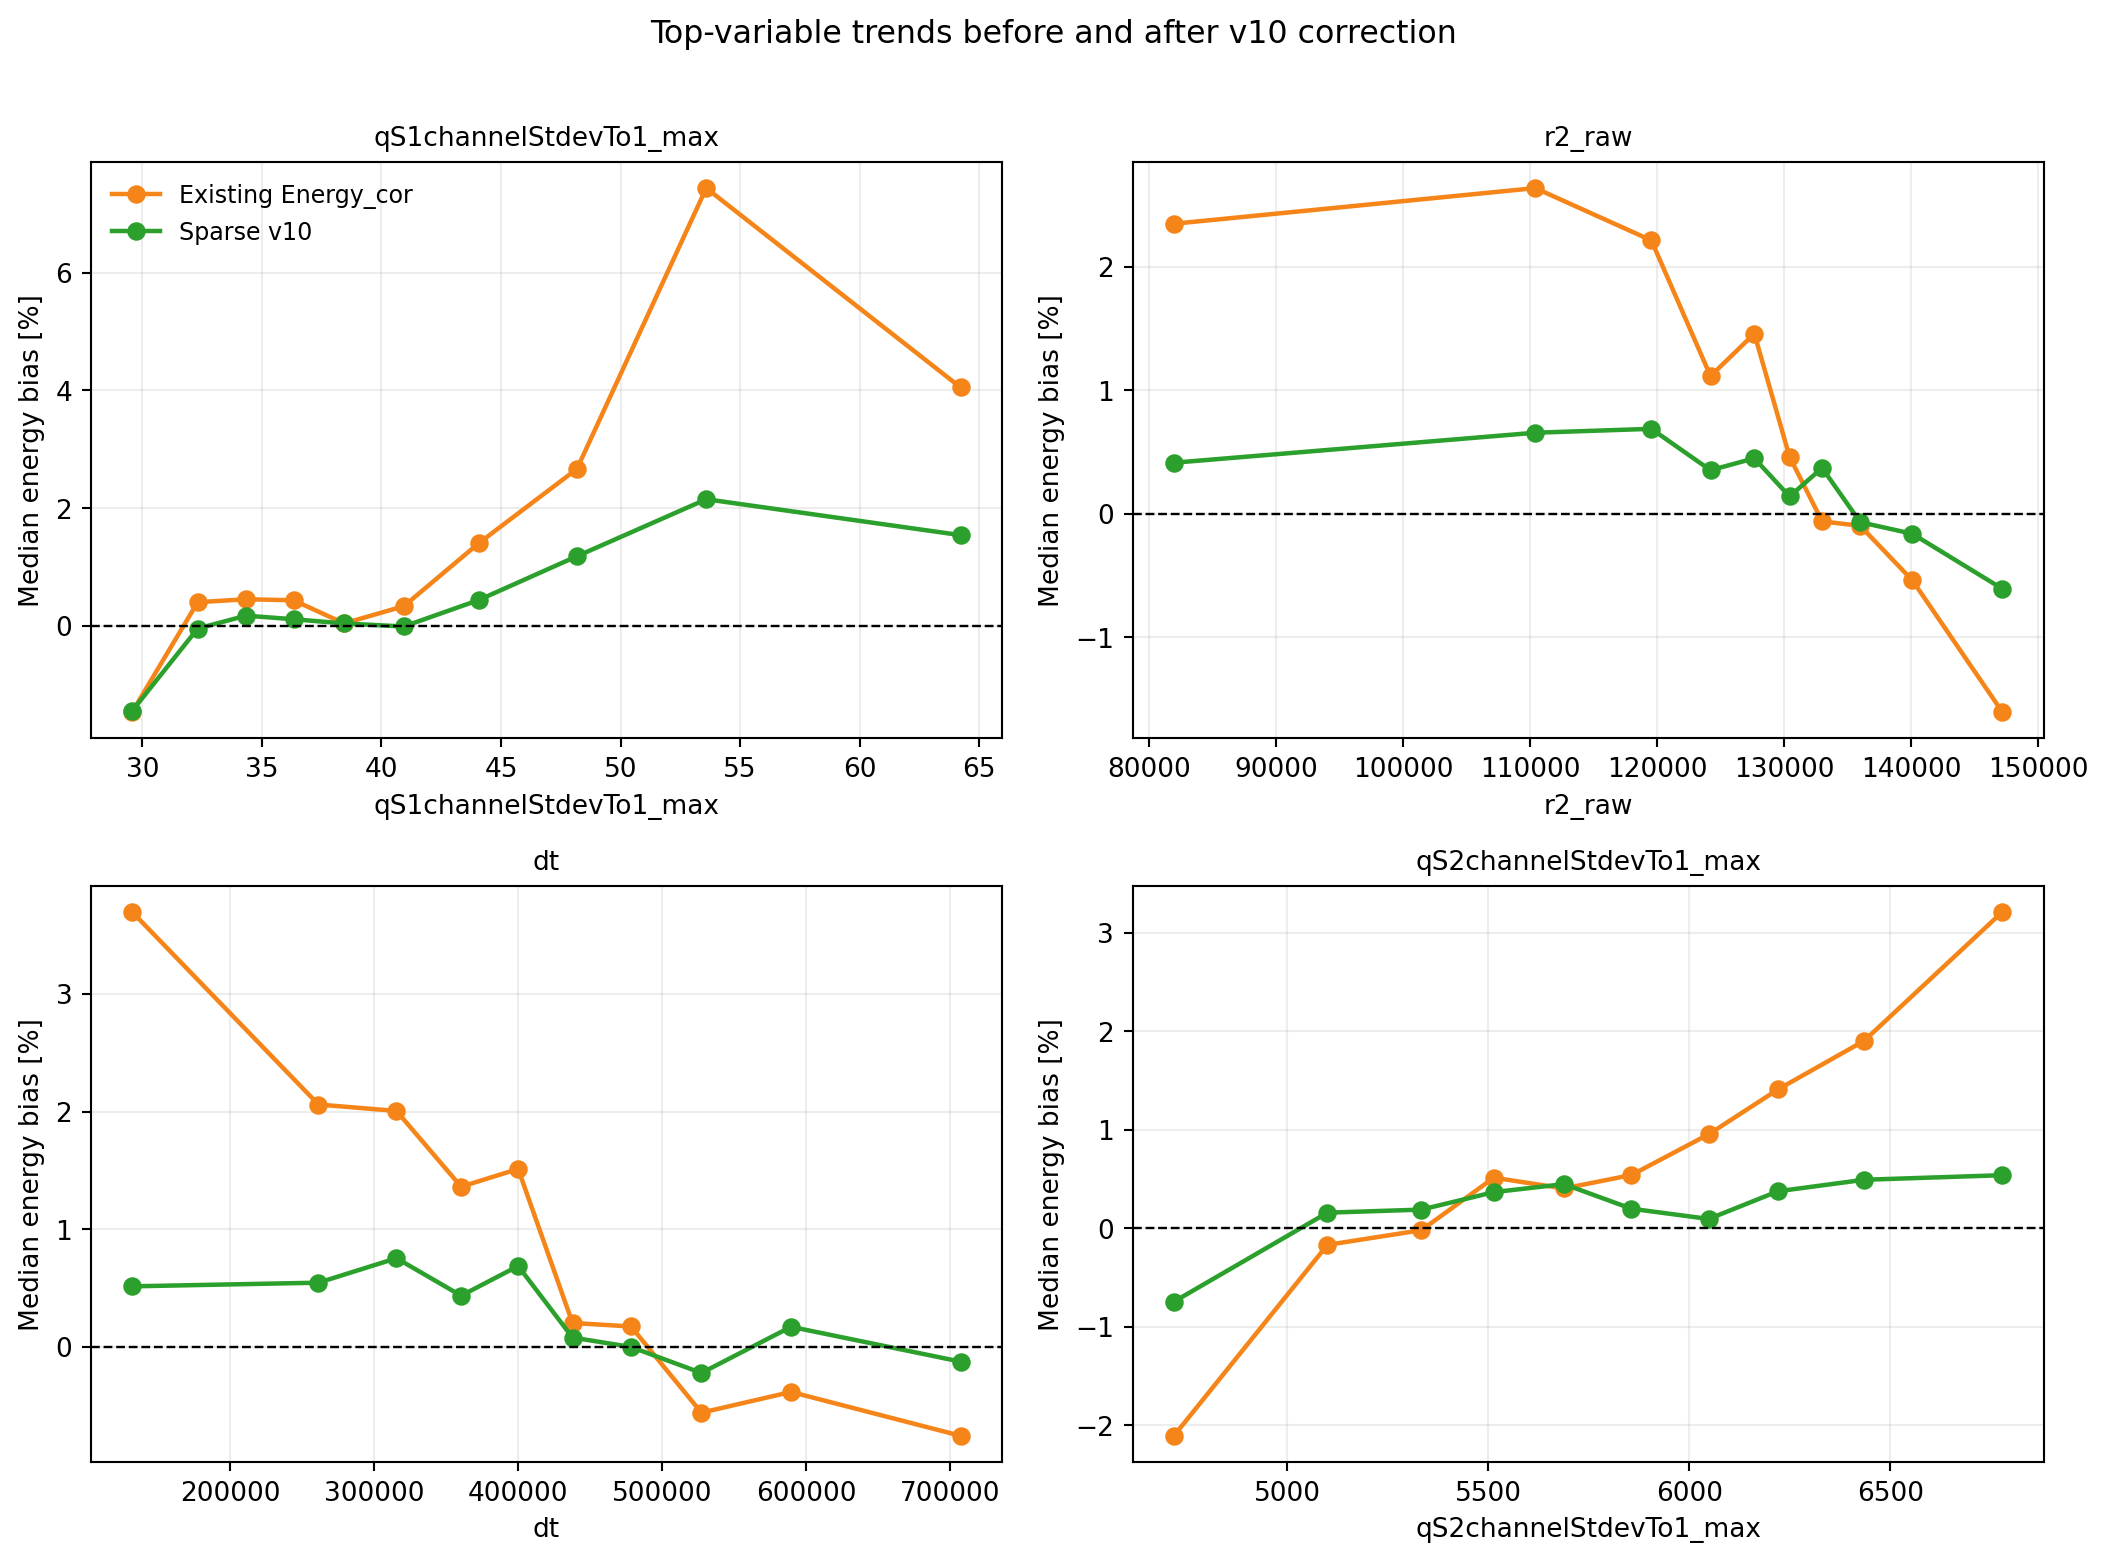
\includegraphics[width=0.98\textwidth]{figures/top_variable_trends.png}
\caption{关键变量等计数分箱中的能量中位偏差。橙色为已有
\var{Energy_cor}，绿色为 v10。v10 明显压低了变量相关趋势，但没有把所有分箱强行固定为零。}
\end{figure}

\section{一维 corrected energy 对比}

\begin{figure}[H]
\centering
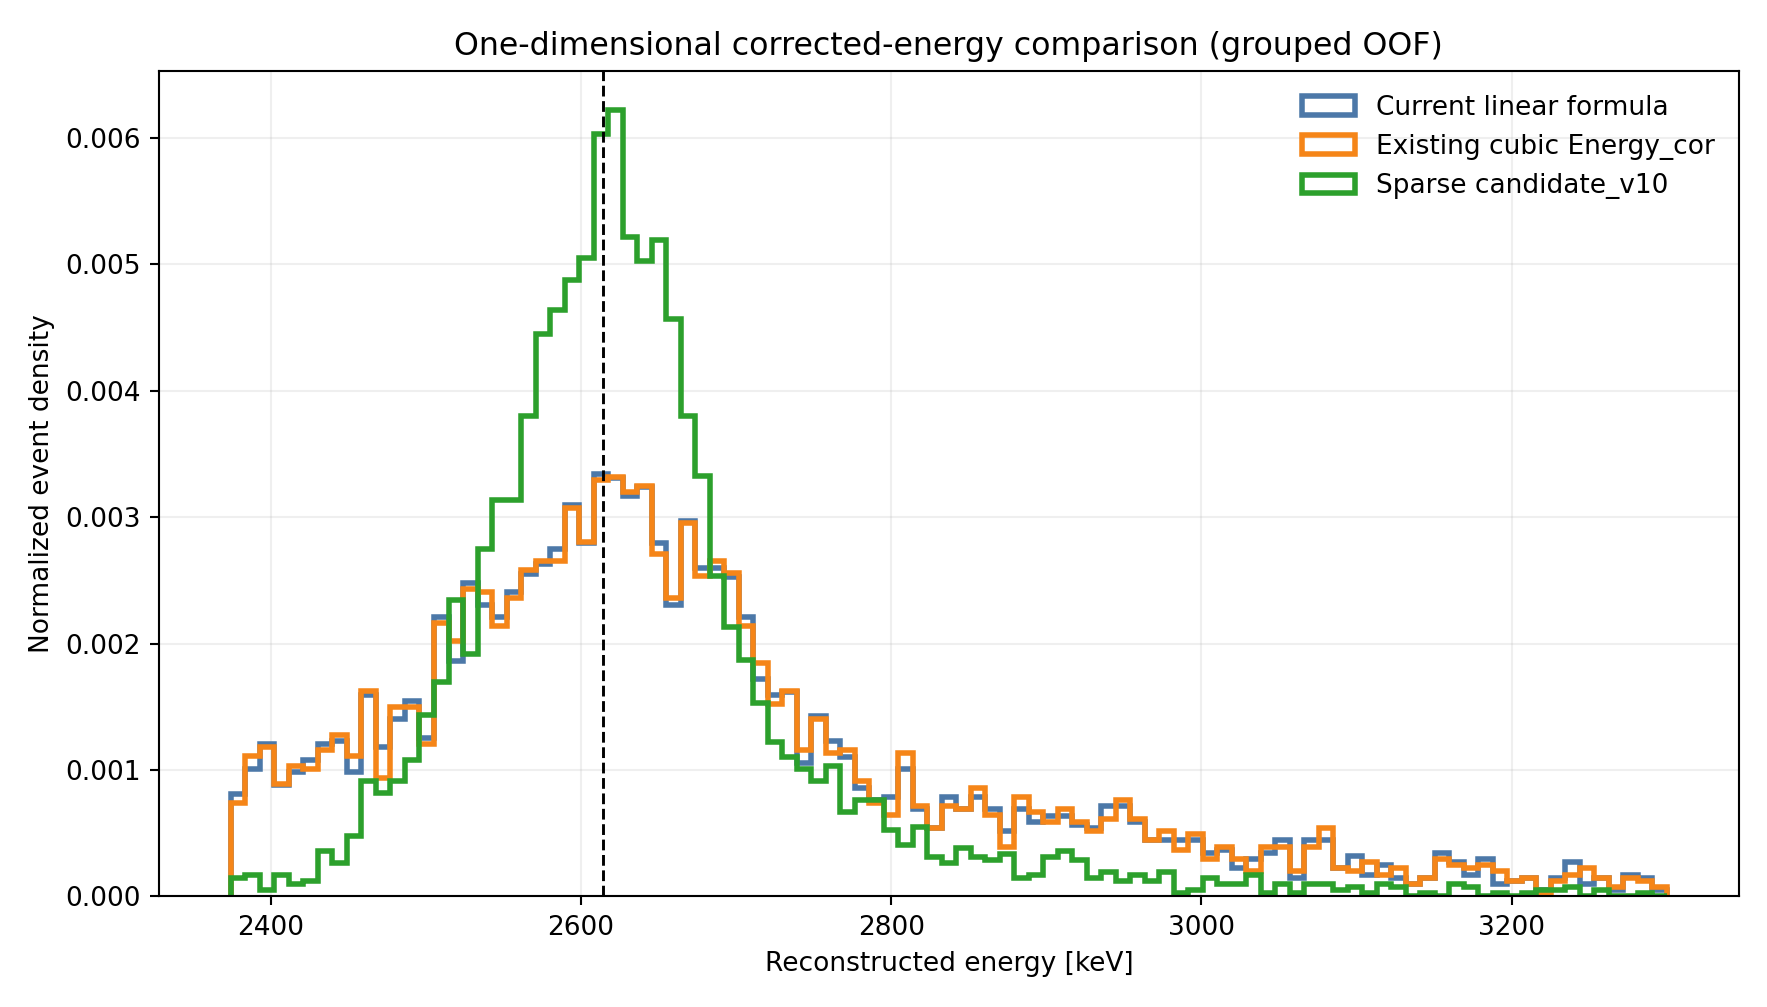
\includegraphics[width=0.96\textwidth]{figures/energy_1d_comparison.png}
\caption{五个外层未见文件块拼接后的 OOF 一维能谱。黑色虚线为
$2614.5~\mathrm{keV}$。v10 的主峰更窄，且高能侧尾部明显减少。}
\end{figure}

\begin{table}[H]
\centering
\caption{合并 OOF 的统一指标}
\begin{tabular}{lrrrr}
\toprule
方法 & 12协议中位 $\sigma/\mu$ & 最差协议 & $R_{68}$ & $R_{90}$\\
\midrule
当前线性公式 & 4.1696\% & 4.3869\% & 6.7861\% & 13.0694\%\\
已有三次 \var{Energy_cor} & 4.1847\% & 4.4404\% & 6.8242\% & 13.1471\%\\
sparse candidate\_v10 & \textbf{2.7698\%} & \textbf{2.8731\%} &
\textbf{3.1059\%} & \textbf{6.7264\%}\\
\bottomrule
\end{tabular}
\end{table}

在相同 OOF 拼接口径下，v10 相对已有三次多项式的峰宽改善为
\begin{equation}
1-\frac{2.7698\%}{4.1847\%}=33.81\%.
\end{equation}
已有三次修正在当前数据与固定协议下没有改善峰宽；这不代表该公式在其原始标定样本上无效，
而是说明它没有消除本批数据中与位置、漂移和通道图样相关的主要波动。

\section{五个未见文件块的稳定性}

\begin{figure}[H]
\centering
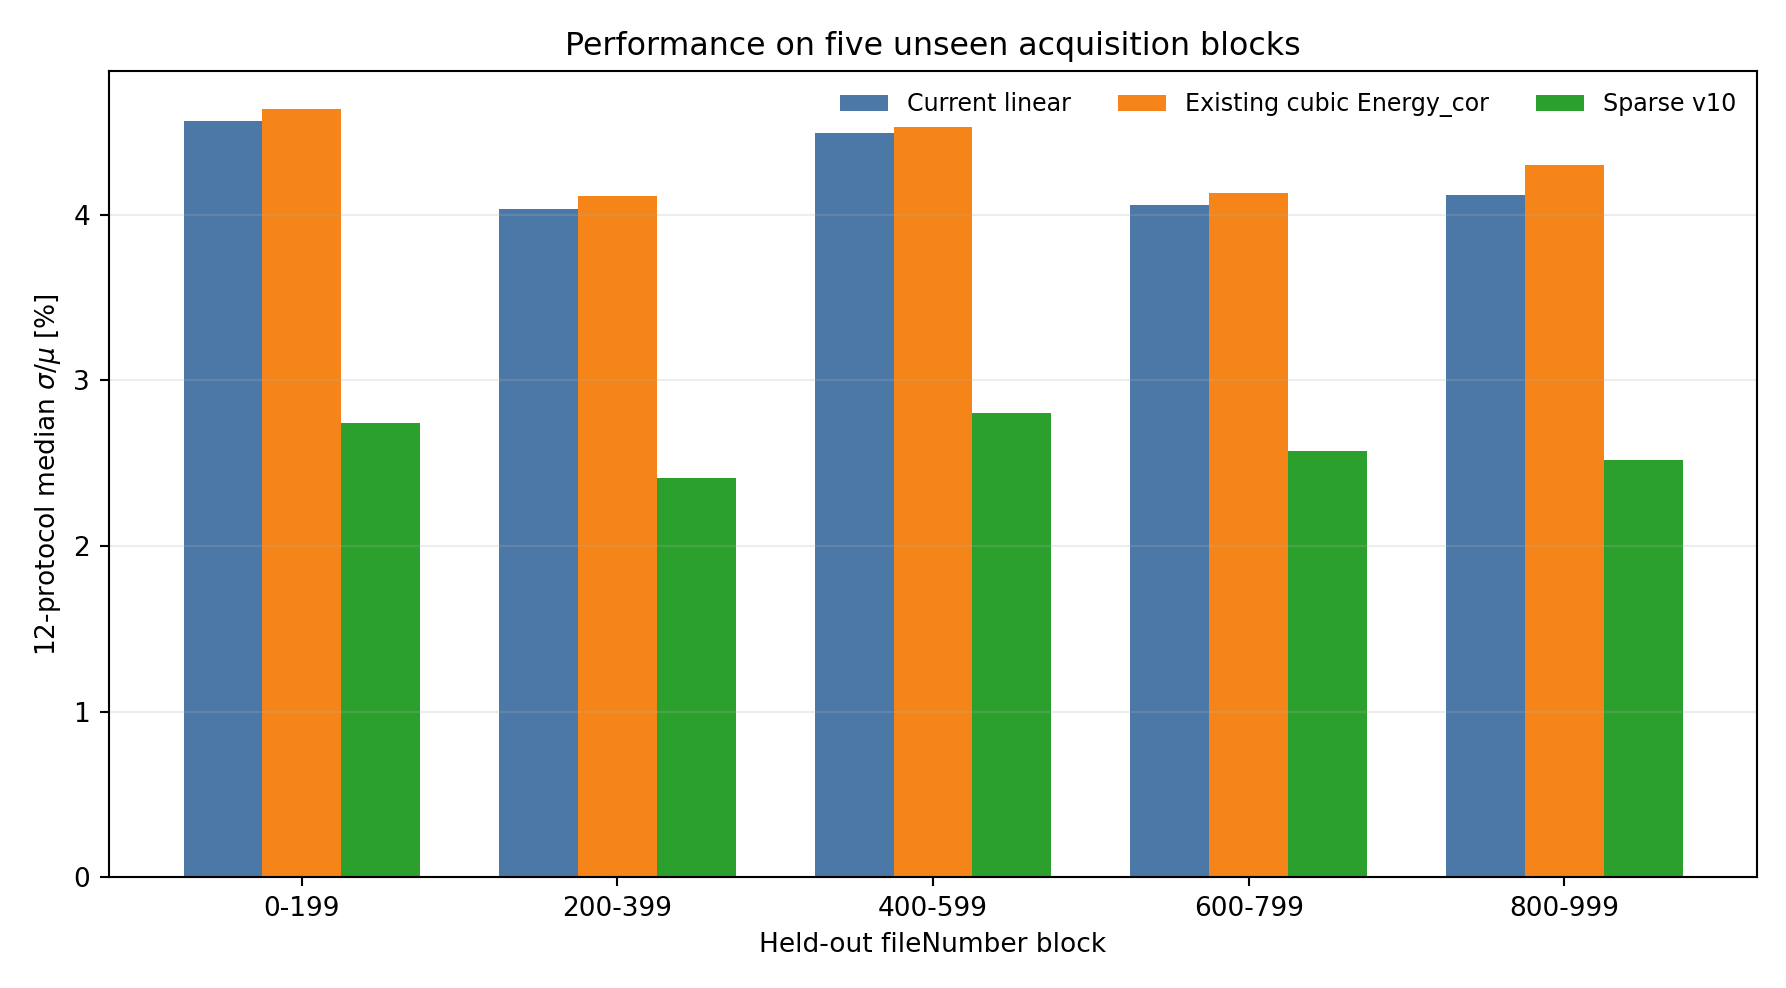
\includegraphics[width=0.96\textwidth]{figures/outer_block_performance.png}
\caption{三个能量路线在五个完整外层测试文件块上的 12 协议中位峰宽。}
\end{figure}

\begin{table}[H]
\centering
\caption{逐外层文件块结果}
\begin{tabular}{crrrr}
\toprule
\var{fileNumber} & 变量数 & 当前线性 & 已有三次修正 & v10\\
\midrule
0--199   & 20 & 4.5616\% & 4.6349\% & \textbf{2.7407\%}\\
200--399 & 30 & 4.0356\% & 4.1127\% & \textbf{2.4100\%}\\
400--599 & 30 & 4.4918\% & 4.5284\% & \textbf{2.8017\%}\\
600--799 & 20 & 4.0605\% & 4.1323\% & \textbf{2.5731\%}\\
800--999 & 20 & 4.1179\% & 4.3011\% & \textbf{2.5159\%}\\
\midrule
中位数 & -- & 4.1179\% & 4.3011\% & \textbf{2.5731\%}\\
\bottomrule
\end{tabular}
\end{table}

五个未见文件块中，v10 均优于当前线性公式和已有三次修正。
相对已有修正的外层中位改善为
\begin{equation}
1-\frac{2.5731\%}{4.3011\%}=40.18\%.
\end{equation}

\section{\texorpdfstring{二维 $x$--$y$ 对比}{二维 x-y 对比}}

\begin{landscape}
\begin{figure}[H]
\centering
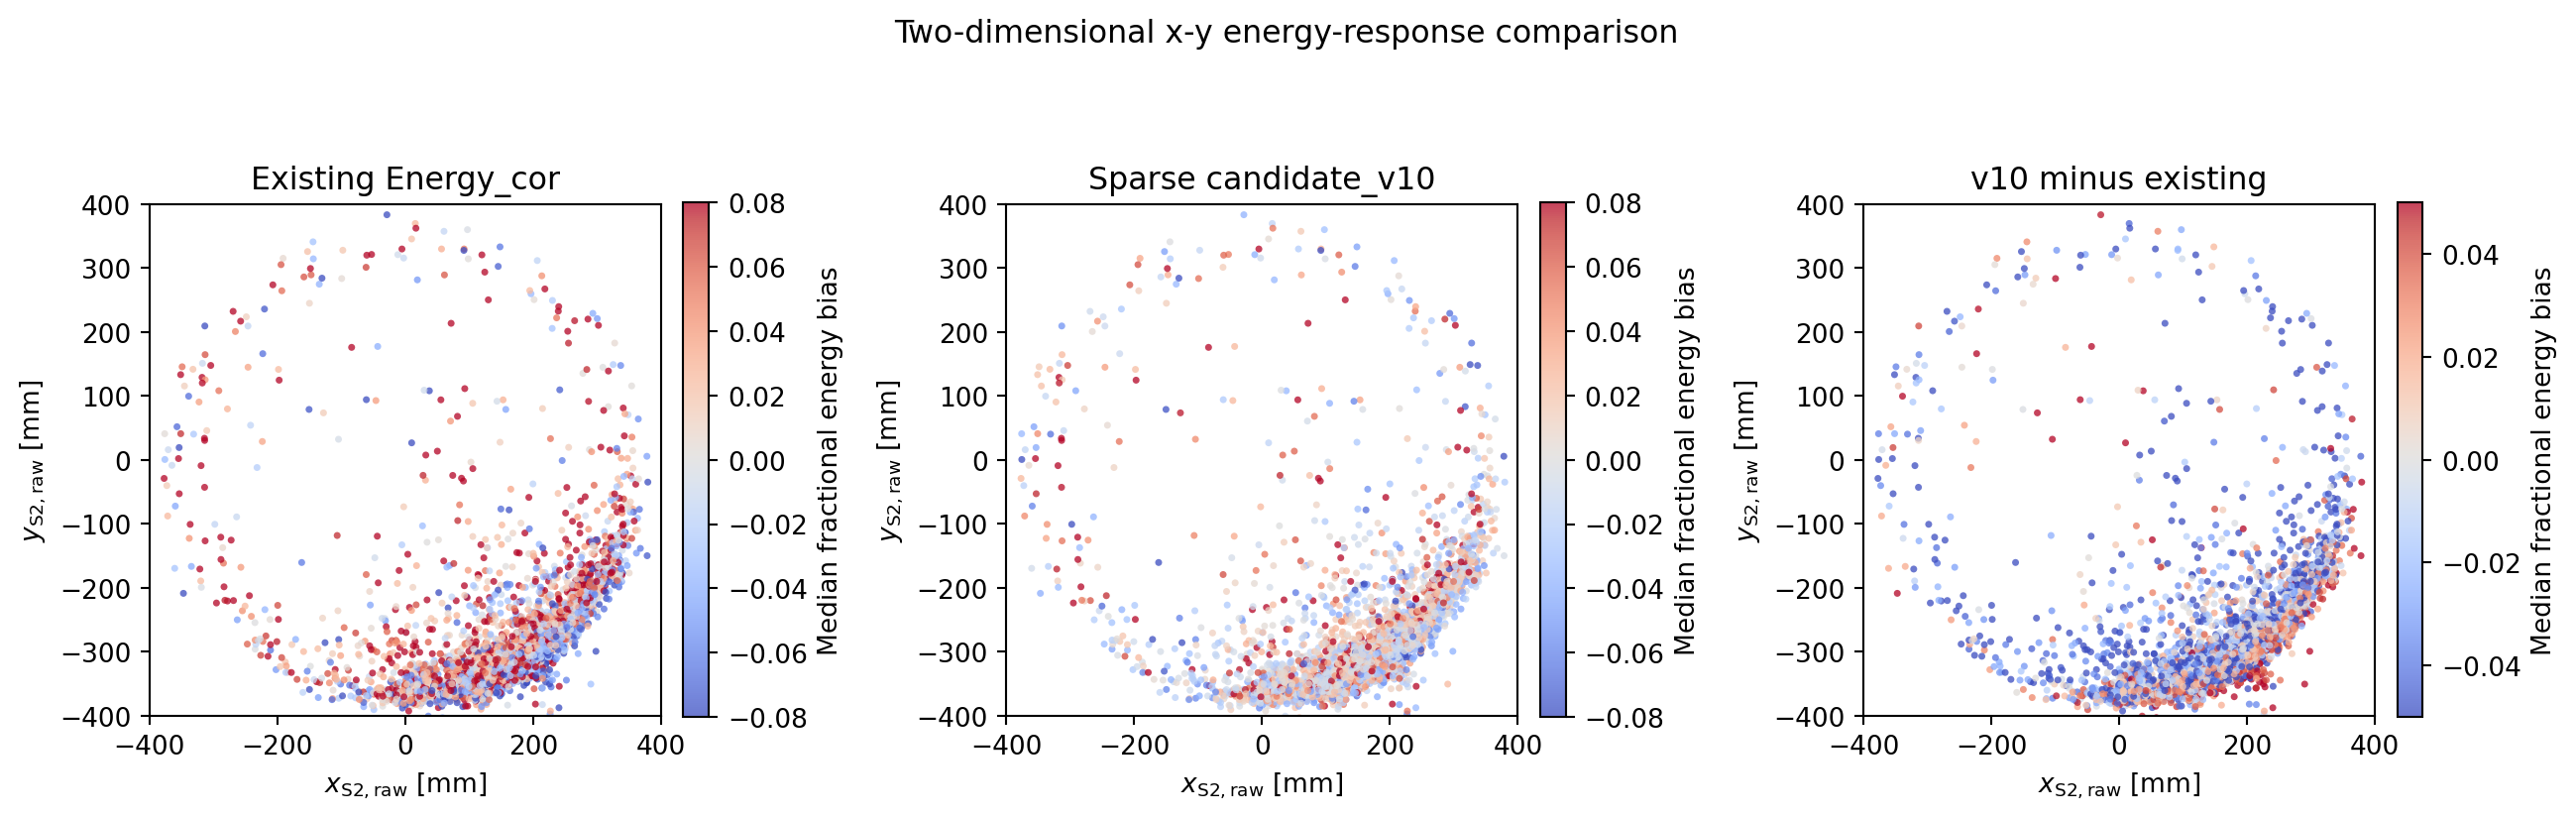
\includegraphics[width=0.96\linewidth]{figures/xy_energy_bias_comparison.png}
\caption{逐事件二维位置对比。颜色表示相对 $2614.5~\mathrm{keV}$ 的能量偏差：
红色为偏高，蓝色为偏低。左为已有修正，中为 v10，右为 v10 与已有修正之差。}
\end{figure}
\end{landscape}

二维图可支持三点判断：
\begin{enumerate}
  \item 已有 \var{Energy_cor} 在横向位置上仍存在明显的红蓝混合和局部结构；
  \item v10 后大部分事件颜色更接近白色，说明位置相关能量偏差整体缩小；
  \item 右图表明修正并非全局常数，而是在底部高统计弧形区域和边缘区域具有更明显的事件级变化。
\end{enumerate}

同时需要注意，上半区域事件较少，二维图在这些位置的统计证据弱于底部高统计区域。
因此，不能仅凭本图宣称整个探测器横截面已经完全均匀。

\section{修正幅度与数值安全}

\begin{figure}[H]
\centering
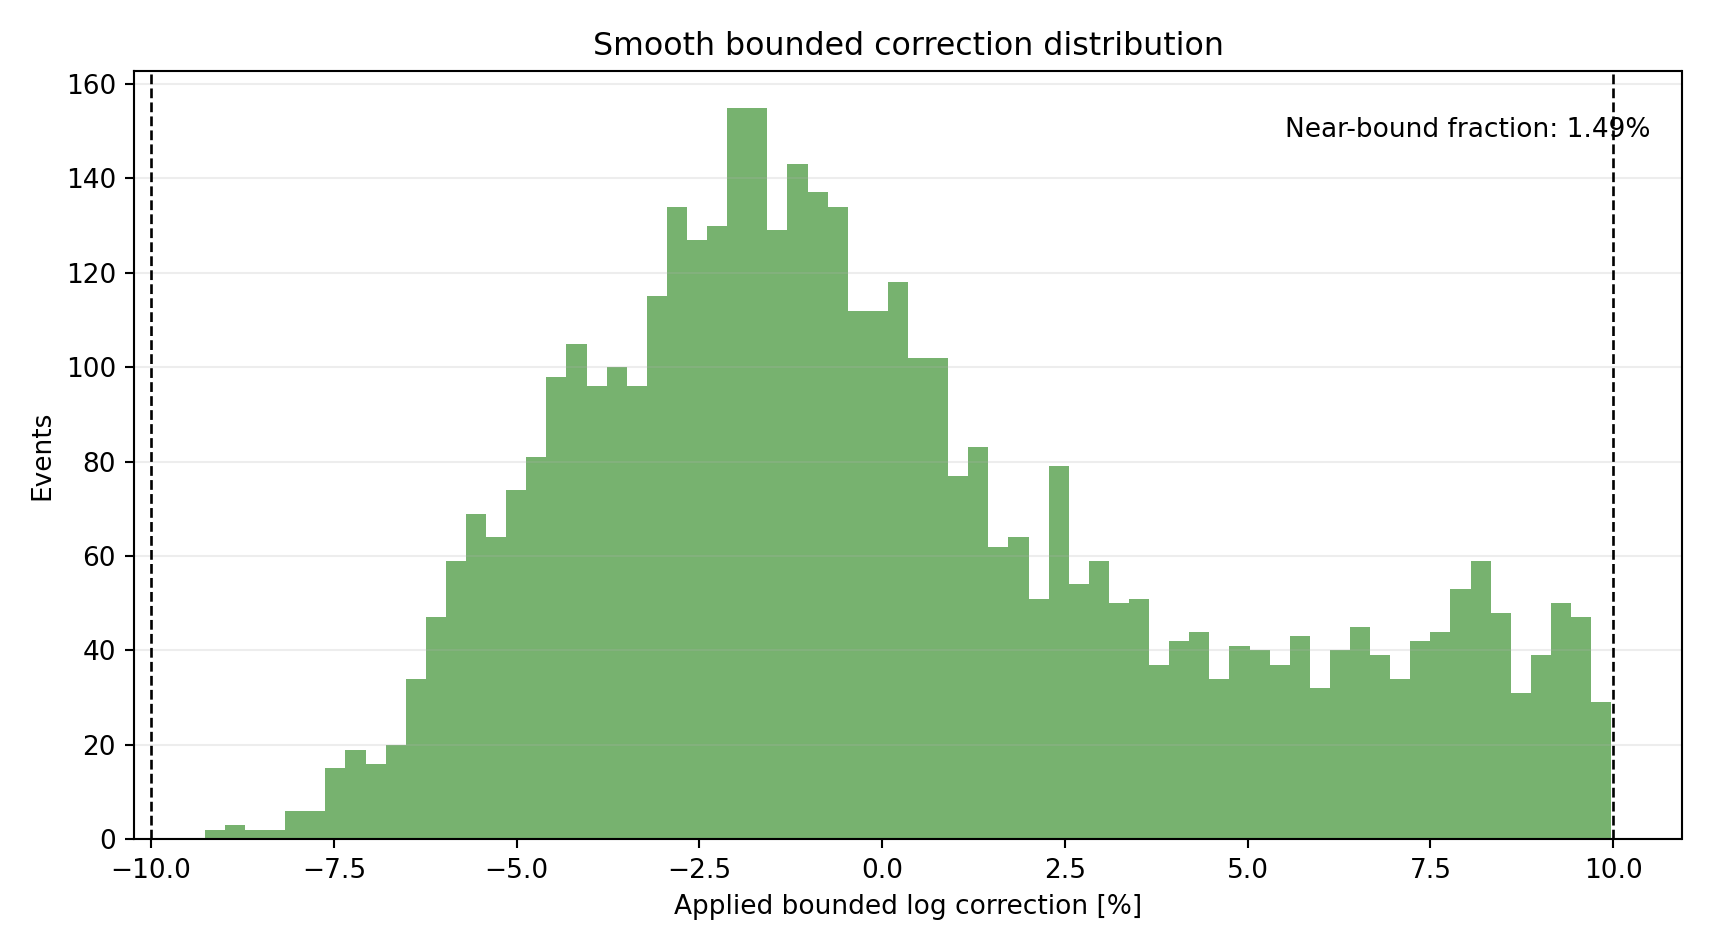
\includegraphics[width=0.92\textwidth]{figures/correction_distribution.png}
\caption{v10 的平滑有界对数修正。虚线为 $\pm 10\%$ 理论边界；
靠近边界的事件比例为 $1.49\%$。}
\end{figure}

所有 4499 个有效事件均得到有限且为正的预测。平滑 $\tanh$ 上限避免了硬截断导致的边界堆积，
并使单事件修正始终满足
\[
|\widehat{\delta}|<0.10.
\]

\section{v9 与 v10 的关系}

\begin{table}[H]
\centering
\caption{模型版本对比}
\begin{tabularx}{\textwidth}{lcccX}
\toprule
版本 & 变量数 & 合并 OOF $\sigma/\mu$ & 外层中位 & 说明\\
\midrule
v9 & 30 & 2.7690\% & 2.6287\% & 完整平滑模型，全部七项门槛通过\\
v10 & 20 & 2.7698\% & 2.5731\% & 嵌套选择变量数，性能基本不损失\\
\bottomrule
\end{tabularx}
\end{table}

v10 的合并 OOF 与 v9 只相差 $0.0008$ 个百分点，说明排名后十个变量对主性能的净贡献很小；
因此 v10 比 v9 更适合向老师解释和进一步控制。

\section{仍然存在的问题}

\begin{enumerate}
  \item \textbf{尚无独立新 run：}所有模型开发与当前证据仍来自 Run 10972；
  \item \textbf{GOF 仍未达到形式接受：}v10 的 12 协议中位拟合
  $p$ 值约为 $3.8\times10^{-39}$，虽然远好于已有修正的
  $4.5\times10^{-124}$，但仍不能称为理想高斯峰；
  \item \textbf{二维覆盖不均：}横向事件在底部弧形区域更密集，上部区域的结论统计较弱；
  \item \textbf{重要性不是因果性：}关键变量说明模型依赖哪些响应代理，不证明具体微观机制；
  \item \textbf{最终20变量仍不是简单解析公式：}当前输出仍需要加载冻结模型。
\end{enumerate}

\section{下一步工作建议}

\begin{enumerate}
  \item 将 v10 冻结为新的老师盲测候选，不再使用 Run 10972 调整变量；
  \item 老师提供新 run 后，一次性输出当前线性、已有三次修正和 v10 三路线；
  \item 在新 run 上重复本报告的 1D、$x$--$y$、关键变量趋势和逐文件块检查；
  \item 若新 run 通过，再研究 12 变量解释模型与 20 变量性能模型的双模型交付；
  \item 若新 run 失败，先保留失败结果，再建立新版本，不能继续称为同一次盲测。
\end{enumerate}

\section*{本阶段完成情况}
\addcontentsline{toc}{section}{本阶段完成情况}

\begin{itemize}
  \item 已完成老师要求的一维 corrected energy 对比；
  \item 已完成 $x$--$y$ 二维逐事件对比；
  \item 已完成关键变量修正前后趋势；
  \item 已给出关键变量排名和五折稳定性；
  \item 已将变量从 30 个减少到 20 个；
  \item 已证明五个未见文件块均优于已有修正；
  \item 已保存冻结模型、逐事件 OOF、变量排序和全部选择账本；
  \item 尚待独立新 run 盲测。
\end{itemize}

\clearpage
\appendix
\section{最终20个变量}

\begin{enumerate}
  \item \var{qS1channelStdevTo1_max}
  \item \var{r2_raw}
  \item \var{dt}
  \item \var{qS2channelStdevTo1_max}
  \item \var{qS1hitStdevTo1_max}
  \item \var{r2_mcpaf}
  \item \var{xS2max_desImageMCPAF_maxS2}
  \item \var{wS1_max}
  \item \var{xS2T_max}
  \item \var{r2_cor}
  \item \var{yS2T_max}
  \item \var{yS2max_desImageMCPAF_maxS2}
  \item \var{qS2hitStdevTo1_max}
  \item \var{rmsCogS1T_max}
  \item \var{xS2Tcor_max}
  \item \var{wS2_max}
  \item \var{yS2Tcor_max}
  \item \var{rmsCogS1B_max}
  \item \var{wS2FWHM_max}
  \item \var{ratioqS1PrePeakSmr_max}
\end{enumerate}

\section{结果文件}

\begin{itemize}
  \item \var{summary.json}：汇总结果与关键变量；
  \item \var{outer_block_metrics.csv}：五个外层文件块结果；
  \item \var{oof_events.csv}：逐事件三路线 OOF 能量；
  \item \var{diagnostic_features.csv}：趋势图和二维图使用的诊断变量；
  \item \var{nested_sparse_selection.json}：每个外层训练池的变量数量选择账本；
  \item \var{final_sparse_selection.json}：最终变量排名与冻结选择；
  \item \var{candidate_v10.joblib}：冻结的稀疏模型。
\end{itemize}

\end{document}
